\documentclass[times, 10pt]{thesisMDH}
\usepackage[ddmmyyyy]{datetime}
\usepackage[pdfborder={0 0 0},colorlinks=true,urlcolor=blue,citecolor=red,bookmarks=false]{hyperref}
\usepackage{float}
\usepackage{makecell}
% \usepackage{indentfirst}
\setlength\parindent{0pt}

\university{University of Science and Technology of Hanoi}
\department{Information and Communication Technology}

\subject{Distributed System}
\thesisTitle{Practical Work 1:\\TCP File Transfer}

\authorOne{Nguyen Phuong Thao}{BI9-212}
\authorTwo{Doan Tuyet Mai}{BI9-162}
\authorThree{Trinh Thao Phuong}{BI9-191}
\authorFour{Phung Kim Son}{BI9-202}
\authorFive{Pham Minh Long}{BI9-146}

\theDate{Hanoi, Feb 2021} 

\begin{document}
\titlePage

\newpage

\mainmatter

\section{Protocol design}
\begin{figure}[H]
    \centering
    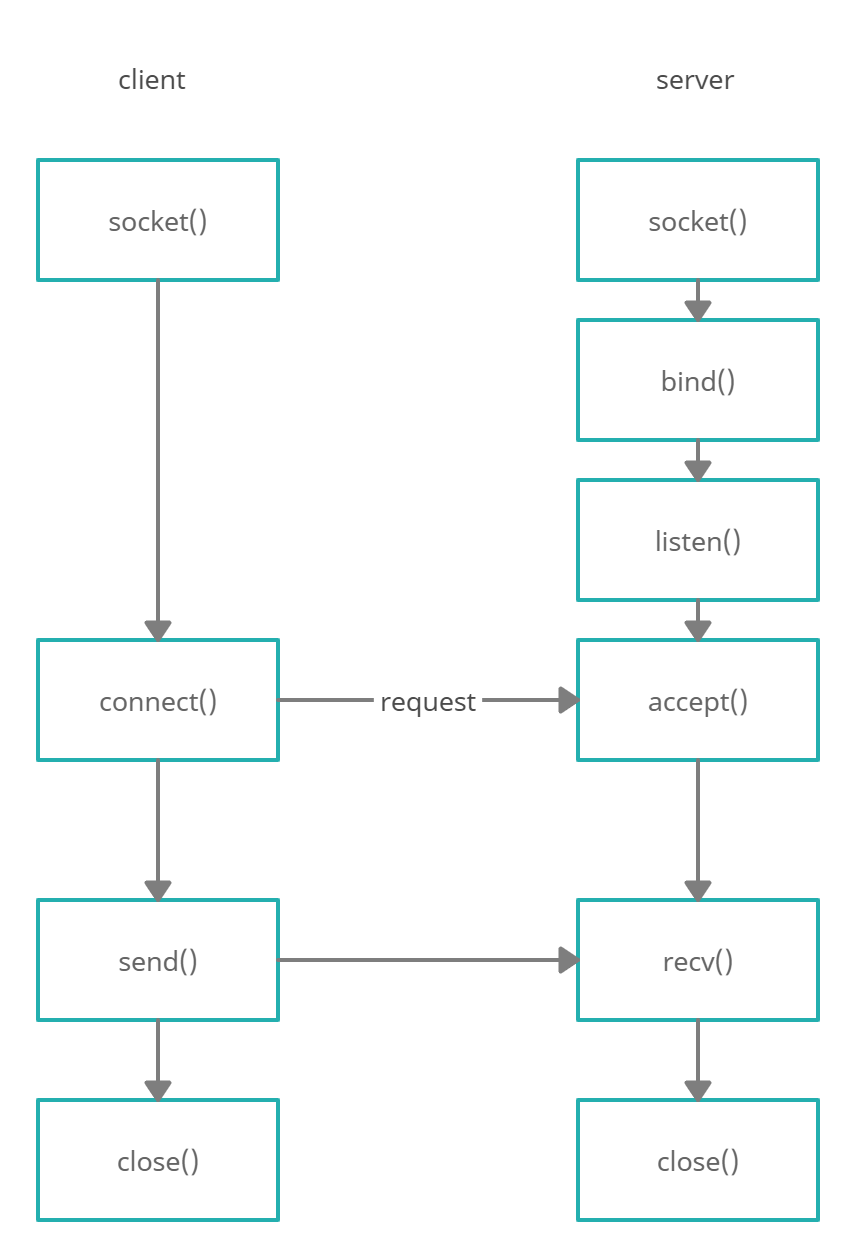
\includegraphics[width = 0.7\linewidth]{images/1-1.png}
    \caption{Protocol design}
\end{figure}
In the server side, at first a socket is created, then it is assigned an address using \texttt{bind()} function and wait for the client. Then in the client side, after a socket is created, the function \texttt{connect()} is used to connect the client to the server. The server uses \texttt{accept()} function to accept the connection from the client. Once connection has succeeded, the client starts to send the file to the connected server and the server receives the file. After transmission is completed, sockets must be closed at both endpoints.
\section{System organization}
\begin{figure}[H]
    \centering
    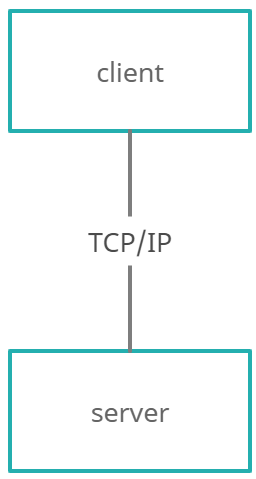
\includegraphics[width = 0.2\linewidth]{images/1-2.png}
    \caption{System organization}
\end{figure}
The server socket will be bind to port with host byte order 12345 after created. It will then listening to data received. The socket will start listening for the connections and accept the connection from the client. Both client and server sending each other data until ones decided to close the socket in open session.
\section{File transfer implementation}
Full code implementation could be found \href{https://github.com/npthao1312/ds2021/tree/master/labwork1/code}{here}, in the \texttt{code} directory.
\subsection{Client-side}
The code for client-side implements these following steps:
\begin{enumerate}
    \item Create a socket, initialize the address of the socket and connect to the server.
    \item Generate a file containing message from the client.
    \item Open the generated file.
    \item Send the generated file to the server.
    \item Close the socket.
    \item The program is stopped.
\end{enumerate}
% In particular 
Firstly, to create a socket:
\begin{lstlisting}
// create socket
int serv = socket(AF_INET, SOCK_STREAM, 0);
\end{lstlisting}
where \texttt{AF\_INET} is an address family that is used to designate the type of addresses that your socket can communicate with, and \texttt{SOCK\_STREAM} indicates that this is a TCP socket.\\[0.5em]
Next, take the hostname from the second argument (argument at the index one) from the command line. From that we could get the address of the server with \texttt{gethostbyname()}. Set the port of the socket the same value as of the server so that they can be connected. Then establish a connection to the server.
\begin{lstlisting}
#include <sys/socket.h>
#include <netdb.h>

struct sockaddr_in ad;
socklen_t ad_length = sizeof(ad);
struct hostent *hep;

// init address
hep = gethostbyname(argv[1]);
memset(&ad, 0, sizeof(ad));
ad.sin_family = AF_INET;
ad.sin_addr = *(struct in_addr *)hep->h_addr_list[0];
ad.sin_port = htons(12345); // translates host byte order to network byte order 

// connect to server
connect(serv, (struct sockaddr *)&ad, ad_length);
\end{lstlisting}
After the client and the server being connected, the file transfer process could be implemented.\\[0.5em]
First, generate a file containing the message:
\begin{lstlisting}
void write_file(char* content){
	FILE *fp;
	fp = fopen("sample.txt", "w");
	fprintf(fp, content);
	fclose(fp);
}
\end{lstlisting}
Then to send the file, first, we read the file that will be sent to have the input of \texttt{FILE} datatype, extract the data with \texttt{fgets()}, then send over the connection with the \texttt{send()} function:
\begin{lstlisting}
#define SIZE 1024
void send_file(FILE *fp, int sockfd){
    int n;
    char data[SIZE] = {0};

    while (fgets(data, SIZE, fp) != NULL){
        // send data over connection
    	if (send(sockfd, data, sizeof(data), 0) == -1){
			perror("Can't send the file!");
			exit(1);
		}
		bzero(data, SIZE);
    }
}

// read generated file
fp = fopen("sample.txt", "r");
if (fp == NULL){
	perror("Error in reading file.");
	exit(1);
}
send_file(fp, serv);
\end{lstlisting}
where \texttt{sockfd} is the the file descriptor associated with the socket.\\[0.5em]
Finally, close the socket and stop the program:
\begin{lstlisting}
// close connection
close(serv);
\end{lstlisting}

\subsection{Server-side}
The code for the server-side implements these following steps:
\begin{enumerate}
    \item Create a socket, initialize the address of the socket and connect to the server.
    \item Generate a new file.
    \item Received the data from the client. 
    \item Open the generated file and write into file.
    \item Close the socket.
    \item The program is stopped.
\end{enumerate}
Create a socket, initialize the address of the socket and connect to the server.
\begin{lstlisting}
 // create the socket
ss = socket(AF_INET, SOCK_STREAM, 0);
// bind the socket to port 12345
memset(&ad, 0, sizeof(ad));
ad.sin_family = AF_INET;
ad.sin_addr.s_addr = INADDR_ANY;
ad.sin_port = htons(12345);
bind(ss, (struct sockaddr *)&ad, ad_length);
\end{lstlisting}
The server start listening for the connections.
\begin{lstlisting}
listen(ss, 0);
\end{lstlisting}
We have a function to write into file.
\begin{lstlisting}
void write_file(int sockfd){
	int n;
	char buffer[SIZE];
	
	FILE *fp;
	fp = fopen("received_sample.txt","w");
	while (1){
		n = recv(sockfd, buffer, SIZE, 0);
		if (n <= 0){
			break;
			return;
		}
		fprintf(fp, "%s", buffer);
		bzero(buffer, SIZE);
	}
	return;
}
\end{lstlisting}
The server accept the connection from the client and write data received into a new file with above write file function. 
\begin{lstlisting}
while (1) {
        // an incoming connection
        cli = accept(ss, (struct sockaddr *)&ad, &ad_length);

        pid = fork();
        if (pid == 0) {
            printf("client connected\n");
            write_file(cli);
            printf("Received file.");
            return 0;
        }
        else {
            // continue the loop to accept more clients
            continue;
        }
    }
\end{lstlisting}
Finally, close the socket and stop the program:
\begin{lstlisting}
// close connection
close(cli);
\end{lstlisting}

\section{Contribution}
\begin{center}
    \begin{tabular}{|l|l|l|}
        \hline
        \textbf{Student} & \textbf{Student ID} & \textbf{Contribution}\\
        \hline
        Pham Minh Long & BI9-146 & Protocol design \\
        \hline
        Phung Kim Son & BI9-202 & System organization \\
        \hline
        Trinh Thao Phuong & BI9-191 & Draw figures \\
        \hline
        Doan Tuyet Mai & BI9-162 & \makecell[l]{Code for file transfer\\Explanation for the implementation of Client-side} \\
        \hline
        Nguyen Phuong Thao & BI9-212 & Explanation for the implementation of Server-side\\
        \hline
    \end{tabular}
\end{center}

\end{document}
